\chapter{Toepassingen}
\vspace{-1cm}\begin{flushright}
{\it `If the facts don't match the theory, \\ change the facts'}\\ A. Einstein
\end{flushright}

\section{Kernfusie en Kernsplijting}
Wanneer een proton $p$ en een neutron $n$ bij elkaar gebracht worden kunnen
ze een verbinding aangaan en een kern van deuterium (`zwaar waterstof') $d$
vormen.
De massa's van $p$, $n$, en $d$ zijn nauwkeurig gemeten:
\begin{eqnarray*}
m_{p} & = & 938,27231 \;\; {\rm MeV/c^{2}} \\
m_{n} & = & 939,56563 \;\; {\rm MeV/c^{2}} \\
m_{d} & = & 1875,61339 \;\; {\rm MeV/c^{2}}
\end{eqnarray*}
De gebruikte eenheid, MeV/c$^{2}$, verdient een nadere toelichting.
Uit de relatie $E = mc^{2}$ volgt dat massa kan worden uitgedrukt in eenheden
van energie gedeeld door $c^{2}$, een constante.
In `MKSA' eenheden is de eenheid van energie de Joule, maar het is ook
mogelijk - en in de hoge-energiefysica gebruikelijk - de elektronvolt, eV, te
kiezen.
Een elektronvolt is de hoeveelheid energie die een eenheidslading oppikt bij
het doorlopen van een potentiaalverschil van 1 Volt.
De eenheidslading (lading van het elektron) is gelijk aan 1,6 $\cdot
10^{-19}$ Coulomb, dus 1 eV = 1,6 $\cdot 10^{-19}$ J, 1 MeV = 10$^{6}$ eV.

% \begin{figure}[h]
% \begin{center}
% \mbox{\epsfxsize=8cm\epsffile{syllabus.pictures/pnbotsing.eps}}
% \caption{}
% \label{f:pnbotsing}
% \end{center}
% \end{figure}

\begin{figure}[ht]
\centering
%\includegraphics[width=.7\textwidth]{syllabus.pictures/pnbotsing}
\epsfig{file=pnbotsing.pdf, width=0.7\textwidth}
\caption{}
\label{f:pnbotsing}
\end{figure}


Omdat de massa van het deuteron (= deuterium-kern) kleiner is 
dan de som van de massa's van
de samenstellende delen, proton en neutron, moet er bij
de vorming van het deuteron dus energie zijn vrijgekomen!
Indien $p$ en $n$ bij elkaar gevoegd worden met verwaarloosbare snelheid, dan
moet gelden dat de energie die vrijkomt gelijk is aan
\begin{eqnarray*}
E & = & m_{p}c^{2} + m_{n}c^{2} - m_{d}c^{2} \\
& = & 2,22455 \;\; {\rm MeV}
\end{eqnarray*}
Deze energie komt vrij in de vorm van een foton:
\begin{displaymath}
p + n \rightarrow d + \gamma
\end{displaymath}
(Een foton is massaloos; het is een kwantum van het electro-magnetische veld,
door Einstein ge\"{\i}ntroduceerd ter verklaring van het foto-elektrische 
effect; we geven het aan met het symbool $\gamma$)
Strikt genomen komt niet alle `ontbrekende massa' ten goede aan de energie
van het foton.
Zelfs als v\'{o}\'{o}r de reactie $p$ en $n$ t.o.v. elkaar in rust zijn, zal
na de reactie het $\gamma$ wegschieten (met de lichtsnelheid) en om
impulsbehoud te
garanderen moet $d$ in tegengestelde richting bewegen, met dezelfde impuls
(zie figuur \ref{f:pnbotsing}).
Door de grootte van de $d$ massa is de met deze impuls samenhangende energie
erg klein.
(Immers, indien $pc \ll mc^{2}$, dan $E = \sqrt{p^{2}c^{2} + m^{2}c^{4}} \simeq
mc^{2}$).

De hierboven besproken reactie is een voorbeeld van kernfusie.
Meer in het algemeen blijkt dat lichte kernen kunnen samensmelten tot
zwaardere terwijl er, net als in het voorbeeld hierboven, energie vrijkomt.
Alle kernen tot en met ijzer kunnen op deze manier via fusie met
`energiewinst' geproduceerd worden (cf. het `opbranden' van sterren).
Omgekeerd blijken zwaardere kernen (een bekend voorbeeld is Uranium) zwaarder
te zijn dan de `som der delen' en komt er bij splijting van deze kernen
energie vrij.

\section{Annihilatie}
In 1932 werd door Anderson in kosmische stralen een nieuw deeltje ontdekt,
met een massa gelijk aan die van het elektron ($e^{-}$), maar 
met tegengestelde en dus
positieve, lading: het positron ($e^{+}$).
Het positron is het anti-deeltje van het elektron. 
Een precieze omschrijving van het begrip anti-deeltje vereist een voltooide
academische natuurkunde-opleiding en meer, hier volstaan we met de
vaststelling dat $e^{+}$ en $e^{-}$ elkaar kunnen `annihileren' 
tot twee (massaloze!) fotonen:
\begin{displaymath}
e^{+}   + e^{-} \rightarrow \gamma + \gamma
\end{displaymath}
(Vraag: Waarom kan de reactie $e^{+} + e^{-} \rightarrow \gamma$, d.w.z.
annihilatie naar \'{e}\'{e}n foton niet plaatsvinden?).
Indien het `annihilatie in rust' betreft zal gelden $E_{\gamma 1} = E_{\gamma
2} = m_{e}c^{2}$ (= 511 keV), waar $E_{\gamma 1,2}$ de energie van de 
fotonen is en $m_{e}$
de elektronmassa (= positronmassa).

\section{Paarcreatie}
Omgekeerd is het ook mogelijk dat een foton een elektron-positron paar
cre\"{e}ert (`paarcreatie'):
\begin{displaymath}
\gamma + Z \rightarrow e^{+} + e^{-} + Z
\end{displaymath}
$Z$ staat hier voor een atoomkern.
Een foton kan niet spontaan in een $e^{+}e^{-}$~-paar vervallen, maar heeft
een ander object nodig om mee te wisselwerken.
Dit object moet elektrisch geladen zijn, anders `voelt' het foton het niet.
De wisselwerking is nodig, omdat het proces $\gamma \rightarrow e^{+}e^{-}$
alleen, energie- en impulsbehoud schendt.

\section{Het Compton-effect}
Het betreft hier de verstrooiing van `elektromagnetische straling' aan 
'materie'.
In het bijzonder zullen we de verstrooiing van electromagnetische straling aan
elektronen bestuderen. Electromagnetische straling bestaat uit fotonen.
Fotonen geven we
aan met het symbool $\gamma$, elektronen met $e$, reactie die we willen 
bestuderen is dus:
\begin{displaymath}
\gamma e ~ \rightarrow ~ \gamma e
\end{displaymath}
Uiteraard moeten we voor de beschrijving van dit proces relativistische kinematica 
gebruiken.

% \begin{figure}[h]
% \label{f:compton}
% \begin{center}
% {\mbox{\epsfxsize=10cm\epsffile{syllabus.pictures/compton.eps}}}
% \end{center}
% \caption[]{Compton verstrooiing, links v\'{o}\'{o}r, rechts na de botsing }
% \end{figure}

\begin{figure}[ht]
\centering
%\includegraphics[width=.7\textwidth]{syllabus.pictures/compton}
\epsfig{file=compton.pdf, width=0.7\textwidth}
\caption[]{Compton verstrooiing, links v\'{o}\'{o}r, rechts na de botsing }
\label{f:compton}
\end{figure}

Zoals in figuur \ref{f:compton} aangegeven, hebben we de volgende situatie:
een foton met impuls $\vec{p}$ en energie $E$ valt in op een elektron in rust, met
massa $m$. Na de botsing heeft het foton impuls $\vec{p}\ ^\prime$ en energie
$E^\prime$. Het elektron heeft na de botsing impuls $\vec{p}_e$ en energie 
$E_e$.
De hoek waaronder het foton verstrooit, m.a.w. de hoek tussen $\vec{p}$ en
$\vec{p}\ ^\prime$ noemen we $\theta$. We gaan nu bepalen hoe groot $E^\prime$
is voor gegeven `bundelenergie' $E$, bij verstrooiingshoek $\theta$.

\noindent
Impulsbehoud: $\vec{p}=\vec{p}\ ^\prime + \vec{p}_e$\\
Impulsoverdracht: $\vec{p} - \vec{p}\ ^\prime = \vec{p}_e$\\
\\
Energiebehoud: $E+m_ec^2=E^\prime + E_e$\\

We rekenen nu de grootte van de impulsoverdracht (gewoon een drie-vector) uit:
\begin{eqnarray}
\label{v:overdracht}
p_e^{2} & = & (\vec{p}-\vec{p}\ ^{\prime})^{2}=\vec{p}^{2}+\vec{p}^{\prime 2}-2\vec{p}\cdot\vec{p}\ ^{\prime}=(E^{2}+E^{\prime 2}-2EE^{\prime}\cos\theta)/c^{2}
\end{eqnarray}

Energiebehoud herschrijven we als: $E_e=(E-E^\prime)+m_ec^2$, waaruit volgt:\\
$E_e^2=(E-E^\prime)^2+m_e^2c^4+2(E-E^\prime)m_ec^2$, met behulp van\\
$E_e^2=p_e^2c^2+m_e^2c^4$ leidt dit tot\\
\begin{eqnarray}
\label{v:overdracht2}
p_e^{2} & = & \{E^{2}+E^{\prime 2}+2(E-E^{\prime})m_{e}c^{2}-2EE^{\prime}\}/c^{2}
\end{eqnarray} 

Invullen van \ref{v:overdracht} in \ref{v:overdracht2} leidt tot 
\begin{displaymath}
E-E^\prime~=~\frac{EE^\prime}{m_ec^2}(1-\cos\theta)
\end{displaymath}
ook te schrijven als
\begin{displaymath}
\frac{1}{E^\prime}-\frac{1}{E}=\frac{1}{m_ec^2}(1-\cos\theta)
\end{displaymath}
Met behulp van de relatie $E=hc/\lambda$ (de energie van een foton van licht 
met een golflengte $\lambda$) leidt dit tot
\begin{displaymath}
\lambda ^\prime - \lambda  = \frac{h}{m_ec}(1-\cos\theta)
\end{displaymath}
De golflengte van het verstrooiende licht verschuift, bij verstrooiing aan een elektron,
dus met een bedrag van orde van grootte $h/m_ec$. Deze grootheid noemen we de
Compton golflengte van het elektron en bedraagt 2,4 $\cdot 10^{-12}$m. 

%\section{Nogmaals het Doppler-effect}
%We hadden gezien dat wanneer een geluidsbron zich naar ons toe beweegt, de toonhoogte zal toenemen
%in vergelijking met de situatie waarin de bron in rust is.
%We zullen nu nogmaals het relativistische Doppler-effect laten zien.
%We hebben gezien dat voor licht per definitie de relatie $E = pc$ moet
%gelden (Deze relatie geldt immers als $v = c$.).
%De Lorentztransformatie voor een lichtstraal die zich in de $x$-richting
%beweegt
%ziet er dan als volgt uit (ga na):
%\begin{displaymath}
%E' = \gamma (1 - \beta) E
%\end{displaymath}
%Dit kunnen we ook schrijven als:
%\begin{displaymath}
%E' = \sqrt{\frac{1 - \beta}{1 + \beta}}E
%\end{displaymath}
%D.w.z. in co\"{o}rdinatenstelsel $S'$ dat met 
%snelheid $\beta c$ in de richting van de lichtstraal
%meebeweegt is de energie van de lichtstraal kleiner (het licht is verschoven
%naar het rood) met een factor
%$\sqrt{\frac{1 - \beta}{1 + \beta}}$,
%Omgekeerd, bewegen we met snelheid $\beta c$ naar een lichtbron toe, dan
%neemt de energie van het
%licht toe met een factor $\sqrt{\frac{1 + \beta}{1 - \beta}}$
%(het licht is verschoven naar het violet).
%Met behulp van de relatie $E = h \nu$ (de energie van een lichtquantum, een
%foton, van licht met frequentie $\nu$; $h$ is een natuurconstante, de
%constante van Planck) volgt:
%\begin{displaymath}
%\nu =  \sqrt{\frac{1 - \beta}{1 + \beta}}\nu
%\end{displaymath}
%precies zoals we ook eerder zagen in vergelijking~\ref{e:doppler}.
%
%\section{Roodverschuiving en het uitdijende heelal}
%Het licht uitgezonden door de vele duizenden melkwegstelsels in het heelal
%blijkt verschoven te zijn naar lagere golflengtes (`roodverschuiving') t.o.v.
%wat verwacht zou worden op basis van standaard spectra.
%M.a.w. deze melkwegstelsels verwijderen zich van onze eigen Melkweg, met een
%snelheid die te bepalen is m.b.v. bovenstaande formule voor relativistische
%Dopplerverschuiving.
%Het heelal dijt uit!
%Deze observatie was een belangrijke bron van inspiratie voor de 'Big Bang'
%theorie van het ontstaan van het heelal.

\section{Deeltjesproductie}

% \begin{figure}[h]
% \begin{center}
% \mbox{\epsfxsize=8cm\epsffile{syllabus.pictures/epbotsing.eps}}
% \caption{}
% \label{f:epbotsing}
% \end{center}
% \end{figure}

\begin{figure}[ht]
\centering
%\includegraphics[width=.7\textwidth]{syllabus.pictures/pppionlab.eps}
\epsfig{file=pppionlab.pdf, width=0.7\textwidth}
\caption{{\sl Voor: een proton vliegt op een stilstaand proton af. Na: het botsingsproduct beweegt in dezelfde richting als het aanstormende proton, maar heeft aan drie-impuls ingeleverd om het} $\pi_0$ {\sl te maken. Merk op dat in deze notatie } $c\equiv 1$.}
\label{f:epbotsing}
\end{figure}


Een spectaculair voorbeeld van een typisch relativistisch effect is de
productie van
`elementaire' deeltjes bij botsingen tussen dergelijke deeltjes.
We geven een voorbeeld:
\begin{displaymath}
p + p \rightarrow p + p + \pi^{0}
\end{displaymath}
of, in een meer gebruikelijke notatie
\begin{displaymath}
pp \rightarrow pp\pi^{0}
\end{displaymath}
Betekenis:
twee protonen botsen op elkaar en er komen uit de botsing weer twee protonen
te voorschijn \textit{plus} een ander deeltje (`er wordt massa
gecre\"{e}erd').
We stellen ons het experiment als volgt voor:
een bundel protonen wordt versneld tot een zekere energie en valt in op een
doelwit bestaande uit protonen\footnote{In de praktijk: waterstof, bestaande uit protonen en elektronen;
elektronen zijn echter veel kleiner dan protonen, zodat het ingaande proton
vrijwel altijd een proton in het waterstof raakt.}.
Gegeven is dat protonen een massa $M_{p}$ = 938 MeV/c$^{2}$ hebben en dat het
$\pi^{0}$ deeltje een massa $M_{\pi}$ = 135 MeV/c$^{2}$ heeft.
De vraag is nu: welke energie, resp. welke impuls moet de protonbundel
minstens hebben, opdat bovenstaande reactie kan verlopen?
In Figuur \ref{f:epbotsing} is de reactie schematisch weergegeven.

Het inkomende proton heeft impuls $\vec{p}$ en energie $E$, die we willen
bepalen.
De overeenkomstige viervector is dus:
$P_{b} = (E, \vec{p}c)$.
Het doelwit heeft een vierimpuls: $P_{d} = (M_{p}c^{2},\vec{0})$.
Om  $P_{b}$ kwantitatief te bepalen realiseren we ons het volgende: vanuit het
zwaartepuntssysteem bezien is de minimale impuls $\vec{p}^{*}$, resp. energie
$E^{*}$ waarbij de reactie kan verlopen \underline{die} impuls waarbij - in het
zwaartepuntssysteem - de deeltjes in de eindtoestand in rust zijn.
Zie Figuur~\ref{f:epcmsbotsing}.

% \begin{figure}[h]
% \begin{center}
% \mbox{\epsfxsize=10cm\epsffile{syllabus.pictures/epcmsbotsing.eps}}
% \caption{}
% \label{f:epcmsbotsing}
% \end{center}
% \end{figure}

\begin{figure}[ht]
\centering
%\includegraphics[width=1.00\textwidth]{syllabus.pictures/pppion.eps}
\epsfig{file=pppion.pdf, width=\textwidth}
\caption{{\sl In het CM-systeem is de som van alle drie-impulsen:} $\sum_i\vec{p}_i = 0$. {\sl Merk op dat in deze notatie } $c\equiv 1$.}
\label{f:epcmsbotsing}
\end{figure}


We kiezen ons assenstelsel z\'{o}, dat $\vec{p}\ ^{*} = (p^{*}, 0, 0)$ en
(dus) $\vec{p} = (p, 0, 0)$.
In het CM-systeem geldt dat de viervector van het bundel-proton gelijk is aan
$P_{b}^{*} = (E^*, p^{*}, 0, 0)$ en die van het doelwit is
$P_{d}^{*} = (E^*, -p^{*}, 0, 0$).
De totale vierimpuls v\'{o}\'{o}r de botsing in het CM-systeem is dus:
\begin{displaymath}
P^{*} = P_{b}^{*} + P_{d}^{*} = (2E^*, 0, 0, 0)
\end{displaymath}
De totale vierimpuls na de botsing in het CM-systeem is, in de `minimale'
situatie die wij beschouwen (met $\widetilde{M}^* = 2M_{p} + M_{\pi}$):
\begin{displaymath}
P'^{*} = (2M_{p}c^{2} + M_{\pi}c^{2},0, 0, 0)
\end{displaymath}
Uit energie- en impulsbehoud volgt
\begin{displaymath}
P^{*} = P'^{*}
\end{displaymath}
en dus:
\begin{displaymath}
E^{*} = M_{p}c^{2} + \frac{1}{2}M_{\pi}c^{2}
\end{displaymath}
$p^{*}$ volgt verder uit: 
\begin{displaymath}
p^{*} = \frac{1}{c}\sqrt{E^{*2}  - M_{p}^{2}c^{4}}
\end{displaymath}
Nu kunnen we de gevraagde energie en impuls, $E$ en $p$, in het Lab-systeem
bepalen via een
Lorentztransformatie.
Dat is de `moeilijke' manier die we eerst zullen illustreren.
Vervolgens doen we het op de gemakkelijke manier.

De Lorentztransformatie die we zoeken moet $-p^{*}$ transformeren naar 0 en
moet de bijbehorende $E^{*}$ transformeren naar $M_{p}c^{2}$:
\begin{eqnarray*}
\left( \begin{array}{c}
M_{p}c^{2} \\
0 
\end{array} \right)
& = &
 \left( \begin{array}{cc}
\gamma & \beta \gamma  \\
\beta \gamma & \gamma
\end{array} \right) 
 \left( \begin{array}{c}
E^{*} \\
-p^{*}c 
\end{array} \right) 
\\
M_{p}c^{2} & = & -\beta \gamma p^{*}c + \gamma E^{*} \\
0 & = & -\gamma p^{*}c + \beta \gamma E^{*} 
\end{eqnarray*}
We hebben in feite slechts \'{e}\'{e}n van deze vergelijkingen nodig om te
vinden: 
\begin{eqnarray*}
\beta & = & \frac{p^{*}c}{E^{*}} \\
\gamma & = & \frac{E^{*}}{M_{p}c^{2}}
\end{eqnarray*}
Nu vinden we $p$ en $E$ uit:
\begin{eqnarray*}
\left( \begin{array}{c}
E \\
pc 
\end{array} \right) 
& = &
 \left( \begin{array}{cc}
\gamma & \beta \gamma  \\
\beta \gamma & \gamma
\end{array} \right) 
 \left( \begin{array}{c}
E^{*} \\
p^{*}c 
\end{array} \right) 
\\
& = & 
\frac{1}{M_{p}c^{2}}
 \left( \begin{array}{cc}
E^{*} & p^{*}c \\
p^{*}c & E^{*}
\end{array} \right) 
 \left( \begin{array}{c}
E^{*} \\
p^{*}c 
\end{array} \right) 
\\
E & = & \frac{p^{*}c^{2} + E^{*2}}{M_{p}c^{2}} \\
pc & = & \frac{2E^{*}p^{*}c}{M_{p}c^{2}} 
\end{eqnarray*}
M.b.v. de eerder gevonden uitdrukkingen voor $E^{*}$ en $p^{*}$ vinden we nu:
\begin{eqnarray*}
\frac{p}{c} & = & \frac{(M_{p} + \frac{1}{2}M_{\pi})\sqrt{M_{\pi}^{2} +
4M_{p}M_{\pi}}}{M_{p}} \\
& = & 777  \;\; {\rm MeV}
\end{eqnarray*}
(Bepaal nu de bijbehorende energie $E$; bepaal de snelheid van de protonen.)

Nu de meer rechtstreekse, gemakkelijkere methode:
\begin{eqnarray*}
P_{b} + P_{d} & = & (E + M_{p}c^{2}, pc, 0, 0 )  \;\; {\rm \; is \; een \; viervector} \\
P_{b}^{*} + P_{d}^{*} & = & (2E^{*}, 0, 0, 0 )  \;\; {\rm is \; de \; getransformeerde \; van \; deze \; viervector}
\end{eqnarray*}
De norm (de `grootte') van een viervector is invariant onder 
Lorentztransformaties, dus:
\begin{eqnarray*}
(P_{b} + P_{d})^{2} & = & (P_{b}^{*} + P_{d}^{*})^{2} \\
(E + M_{p}c^{2})^{2} - p^{2}c^{2} & = & 4E^{*2}
\end{eqnarray*}
(Let op het $-$ teken!)
Uitwerken hiervan levert hetzelfde resultaat als hierboven (ga na).

%%% Local Variables: 
%%% mode: latex
%%% TeX-master: "Toepassingen"
%%% End: 
